\setchapterpreamble[u]{\margintoc}
\chapter{Findings: Mobile Analytics Tools and their Artefacts}~\label{chapter-tools-and-their-artefacts}
This chapter covers two of the six perspectives, \emph{i.e.} using and improving mobile analytics tools. The primary evidence comes from both the app-centric and the tool-centric case studies, augmented with material from grey data and grey literature.

The evidence has been analysed and prioritised to keep the chapter relatively succinct and on topic. 38 discrete themes (L1 themes) emerged in the analysis of the evidence, of these the 18 with strongest support in terms of the evidence are included here, the rest would benefit from further work. The L1 themes included in this chapter have be aggregated into four higher-level (L2) themes: design (\secref{section-design}), fit-for-purpose (\secref{section-fit-for-purpose}), utility (\secref{section-utility}), dependability (\secref{section-dependability}). Figure \ref{fig:analytics-tools-and-their-artefacts-fishbone-diagram} illustrates the top L1 themes and their primary higher-level (L2) theme.

\begin{figure*}
    \centering
    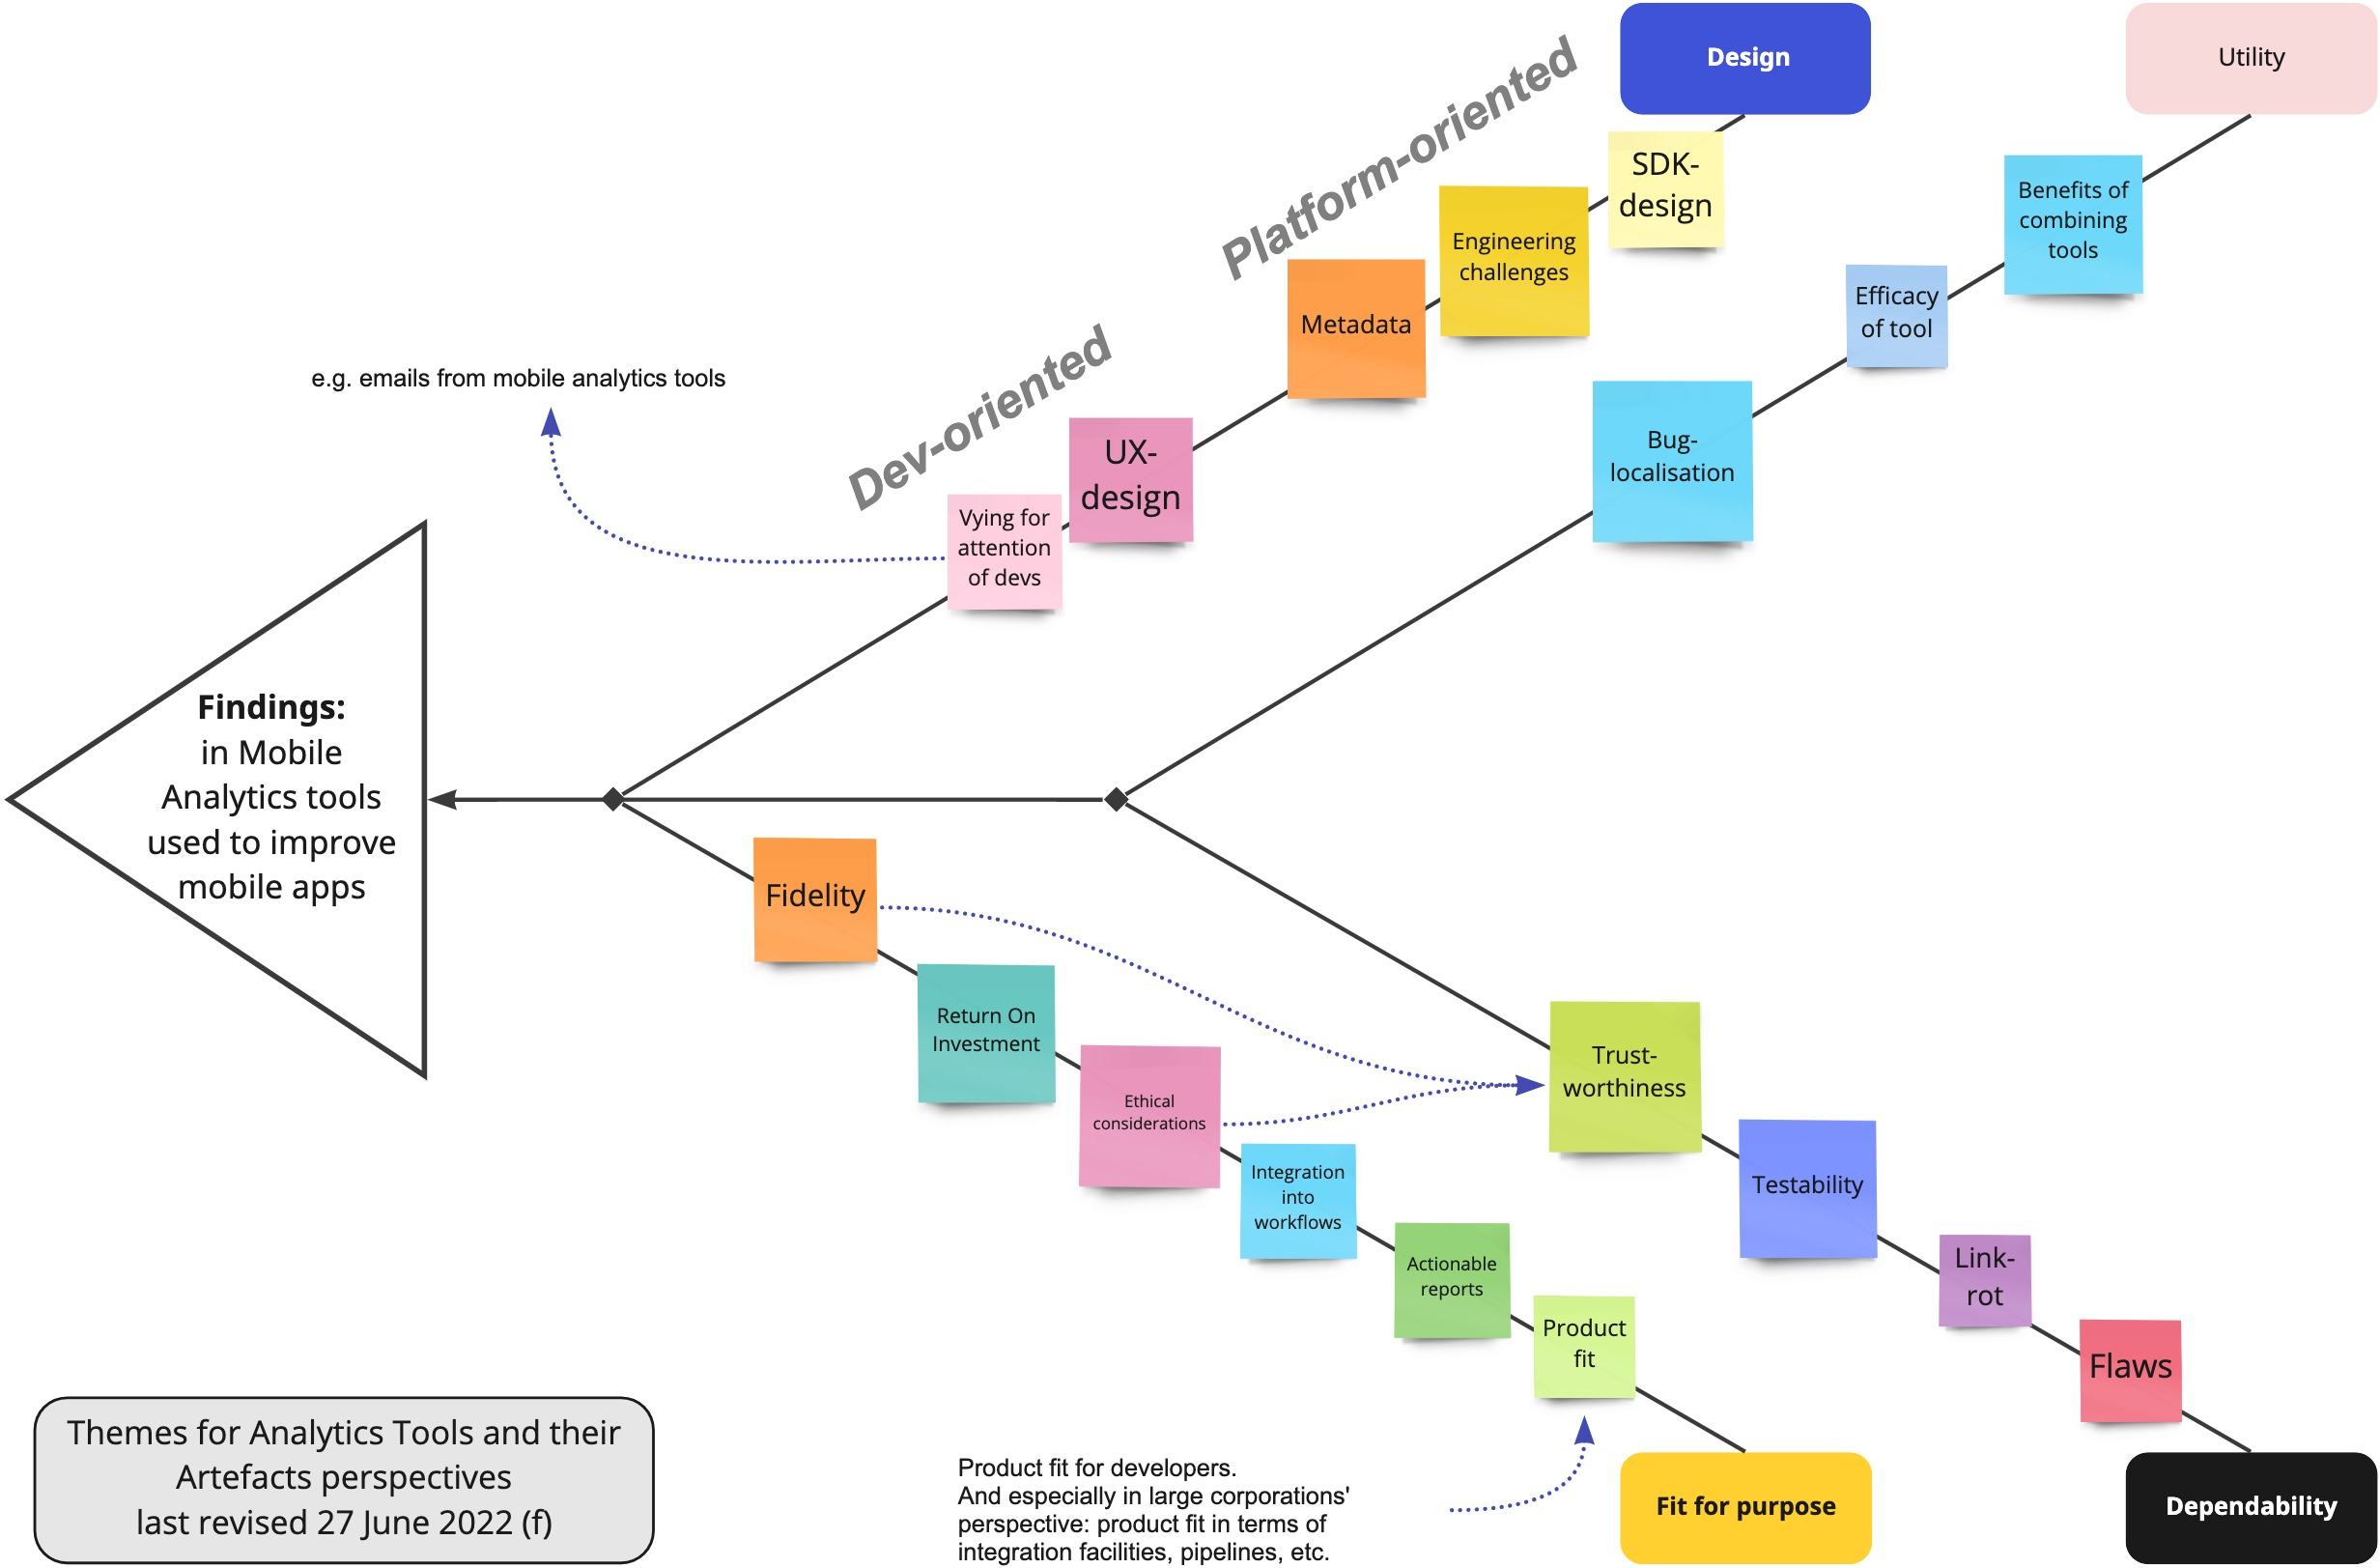
\includegraphics[width=\linewidth]{images/rough-sketches/analytics-tools-and-their-artefacts-fishbone-diagram-27-jun-2022f.jpeg}
    \caption{Analytics Tools and their Artefacts Fishbone Diagram\\Source: \href{https://miro.com/app/board/uXjVOtIsyWo=/?share_link_id=293061080490}{Miro}}
    \label{fig:analytics-tools-and-their-artefacts-fishbone-diagram}
\end{figure*}

\section{Design}~\label{tata-design-section}
Design emerged as by far the most pertinent topic for the mobile analytics tools. There are two key, connected facets: 


\begin{itemize}
\item the design of the on-device \Gls{sdk}, including addressing various engineering challenges and deciding on the meta-data to collect; and 
\item UX design to engage the developers to actually use the results of the mobile analytics [effectively].
\end{itemize}

The design of the on-device SDK is important because any in-app SDK needs to integrate easily in to the mobile app, and platform-level analytics need to be seamless and collect sufficient pertinent information to be useful for the app developers. They also need to be robust and timely in terms of collection, transmission, and processing of the underlying data in order for developers to have timely access to the results.

Mobile Analytics tools need to be used to be effective, and the user experience of the developers who use these tools where \emph{``developers’ needs are characterized by efficiency, informativeness, intuitiveness, and flexibility of the tool.''}~\sidecite[][p. 104]{kuusinen2016_flow_intrinsic_motivation_and_developer_experience_in_sw_eng}. Where using a tool is rewarding for the developers they are likely to use the tool more~\sidecite[][p. 260]{kuusinen2016_are_sw_devs_just_users_of_devt_tools_etc}.

These tools are a subset of software trying to get a developer's attention and they need to fit within a larger context. The tools need to surface (make visible) functionality and capabilities that align with the motivation(s) of the developers~\sidecite[][p. 2]{zaina2021_ux_information_in_the_daily_work_of_an_agile_team}.

\myindex{Fabric Crashlytics} is an archetypal example of how a mobile analytics tool can be designed to serve developers well. The product team developed it from the ground up, starting with excellent crash reporting, to provide developers with timely, actionable, attractive, and useful reports. This led to it becoming one of the top three mobile analytics tools for both iOS and Android within 10 months of being launched~\sidecite{___answersblog_2015_may_crashlytics-no1-in-performance}. % See also https://web.archive.org/web/20151203150947/http://fabric.io/blog/crashlytics-answers-named-top-mobile-sdks
First Twitter acquired it and then Google did; they subsequently integrated it into \myindex{Firebase Analytics} which is the most popular mobile analytics service for Android apps currently. 

It exemplified good design in terms of the SDK as it collected pertinent data developers found useful without requiring significant effort by the developers. The development team who created the SDK and the product had used their frustrations from using other analytics software as a catalyst to create Crashlytics. 

Similarly the user-interface of Crashlytics was slick from the outset and quickly adopted by app developers through presenting the analysis of the data the SDK had collected. It was designed from the outset to be actionable save \emph{`developers from information overload or ``analysis paralysis'''}~\sidecite{burke2014_wayne_chang_interview}.

Developers found it useful, it was free of charge, and the product continued to evolve and improve rapidly, for example by adding a general purpose mobile analytics service, called Answers, to Crashlytics that, in their words: \emph{``Before Answers, developers had to wade through mountains of data about their apps to find what they were looking for. We wanted to fix this, so we went to the drawing board and set out to build a mobile analytics solution you didn’t need to analyze.''}~\sidecite{___answersblog_2015_may_crashlytics-no1-in-performance} 

Platform-level analytics provides an outsider's perspective on the behaviour of mobile app, in contrast to in-app analytics that provides an insider's perspective. In this research Google's Android Vitals provides the platform-level analytics as it has the largest reach of any platform-level analytics across the widest range of devices. The platform provides users the ability to allow or deny analytics to be sent from their device. Apple's iOS (and MacOS) ask the user explicitly~\sidecite{apple_ios_share_diagnostics}, Android does not - users need to find the setting and opt-out~\sidecite{google_play_share_usage_and_diagnostics_info_with_google}. % See also https://chefkochblog.wordpress.com/2018/02/09/how-to-disable-android-usage-diagnostics-sharing/ I've not referenced this as they don't provide evidence of the default settings.

Mobile Analytics tools vie for attention against a plethora of other developer-oriented tools, project demands, \emph{etc.} Developers need to be enticed into using the tools and then retained on an ongoing basis to meet the objectives of the providers of the mobile analytics services.

\subsection{SDK design}~\label{section-sdk-design}
Any mobile analytics SDK needs to be designed to collect relevant data and forward that data so it can be processed, analysed, and reported on. The design of the client-side SDK affects many aspects of the data collection which then feeds subsequent stages in the processing of the data to provide the mobile analytics.

\newthought{Programming language support: } 
Mobile apps can be written in several programming languages, including Java, C++ and others. While many mobile apps are written in a single programming language some use several programming languages, for instance Kiwix Android combines Java, Kotlin, and C++. 
% More reading on Cordova's demise: https://medium.com/codex/the-sunset-of-apache-cordova-alternatives-for-cross-platform-mobile-development-in-2022-9da34234c992

Mobile analytics SDKs, in turn, support one or more of the programming languages. If they do not support the programming languages then they may not be able to obtain or provide analytics for elements written in the unsupported programming languages. For C and C++ code in particular, the app developers generally need to explicitly configure the code and the build process to incorporate the relevant mobile analytics SDK if it's available. % For a counterexample Fabric Crashlytics claimed their SDK was very easy to integrate https://web.archive.org/web/20151019132428/https://crashlytics.com/blog/the-wait-is-over-launching-crashlytics-for-android-ndk



\newthought{SDK initialisation: } 
The SDK needs to be initialised as early as practical each time the app is started (or restarted) if it's to capture pertinent information (including crashes that occur when the app starts or restarts): \emph{``for these products is that it would have to be wired in super early in the App's lifecycle, to (say) allow Crashlytics to capture crashes that happen early on''}~\sidecite[][issuecomment-635498836]{paularius2018_initialise_firebaseapp_without_google_services_json_issue_66}. 
% The discussion continued in https://github.com/firebase/firebase-android-sdk/issues/187 then returned to issue 66. And see also https://stackoverflow.com/questions/54927957/unable-to-make-firebase-work-for-a-non-gradle-build-missing-google-app-id-fire/55006495#55006495
For mobile analytics SDKs this has led to the developers of the SDK finding and implementing mechanisms to initialise their SDK in innovative (and unusual) ways, for instance Firebase uses a ContentProvider~\sidecite{stevenson2016_how_does_firebase_initialize_on_android}. Note: this does not always work, as reported in \sidecite{reddy2022_crashlytics_fails_to_track_app_startup_crashes}. When the SDK initialises it obtains various meta data about the app and the device. 
% \url{https://github.com/firebase/firebase-android-sdk/issues/66} % Found via https://lightrun.com/answers/firebase-firebase-android-sdk-initialize-firebaseapp-without-google-servicesjson

\newthought{Data automatically collected by SDKs: }
The mobile analytics SDKs have collected data automatically for years, the developers do not need to write additional code to collect this data. The data includes meta-data about the device and version of the platform. Depending on the SDK it may also collect demographic data, sensor data such as the geo-location, other data such as other apps that are installed, and various events that occur including network requests and responses. The data collected is covered shortly in \ref{section-meta-data}.

Any of these data elements \textit{may} help developers to improve their software, however, use of this data may be considered a privacy risk, particularly for end-users and may lead to ethical conundra for the development team and their organisation, see \ref{aiu-ethics-and-pii-topics}.

\newthought{Runtime activities for the SDK: } 
When the SDK is running, which they do in the background without being visible to the user of the app, they are responsible for the safekeeping and transmission of the collected data. Some collect data automatically, or autonomously. For example, Sentry's in-app SDK collects `automatic instrumentation'~\sidecite{sentry2021_mobile_vitals_four_metrics_every_mobile_developer_should_care_about}, and Android Vitals collects usage data, app crashes, and ANRs automatically.

At least some of the SDKs store analytics data locally on the device on an interim basis, the stored data would be removed once it had been successfully transmitted. Various SDKs limit the number of items they store. The SDKs also vary in how and when they transmit the data and on their behaviour if there isn't a suitable network connection to transmit the data.


\newthought{In-app analytics support for detecting ANRs: } 
At the start of the research in-app analytics SDKs were not able to measure ANRs which meant Android Vitals was the primary source of \Gls{anr} analytics for Android app developers. Subsequently, an opensource utility called \myindex{ANR watchdog} was released that uses a watchdog timer to detect ANRs~\sidecite{salomonbrys_github_anr_watchdog}. 
Investigating it in depth was beyond the scope of the immediate research, nonetheless Sentry used that code as a basis for their ANR reporting (\href{https://github.com/getsentry/sentry-java/blob/3f8d7b1cc869bb056c9db99b459e43f6c375784a/sentry-android-core/src/main/java/io/sentry/android/core/ANRWatchDog.java}{sentry-android-core...ANRWatchDog.java}). 

Note: Google has subsequently added a mechanism to enable apps to obtain information about previous ANRs when the app next started. The method is \index{getHistoricalProcessExitReasons}\href{https://developer.android.com/reference/kotlin/android/app/ActivityManager#gethistoricalprocessexitreasons}{\texttt{getHistoricalProcessExitReasons()}}~\sidenote{The source code is available online: \href{https://android.googlesource.com/platform/frameworks/base/+/master/core/java/android/app/ApplicationExitInfo.java}{android.googlesource.com/ ..... /ApplicationExitInfo.java} and provides more details of the design and the data structures.}, added in \href{https://developer.android.com/about/versions/11}{Android 11}, API level 30.
% Various discussions and explanations of using this API follow:
% https://commonsware.com/R/pages/chap-dataaccess-002.html - possibly the best and clearest code examples with explanations.
% Announcing the new functionality in 2021 https://firebase.blog/posts/2021/11/whats-new-at-Firebase-Summit-2021
% https://medium.com/@yangweigbh/monitoring-app-termination-on-android-11-97d514a3f9 
% Facebook's SDK to obtain cached ANRs https://developers.facebook.com/docs/reference/androidsdk/current/facebook/com/facebook/internal/instrument/anrreport/anrhandler.html/ and https://github.com/facebook/facebook-android-sdk/blob/5fe6e2a9d7056a17f54c1cae13e00788723d34f6/facebook-core/src/main/java/com/facebook/internal/instrument/anrreport/ANRHandler.kt
%
At the time of writing, Firebase Analytics uses this mechanism to obtain the \Gls{anr} and other app exit data~\sidenote{\href{https://github.com/firebase/firebase-android-sdk/blob/73131b69b0134456441e7fa218964b6a766fcec7/firebase-crashlytics/src/main/java/com/google/firebase/crashlytics/FirebaseCrashlytics.java}{github.com ..... FirebaseCrashlytics.java}}.


\subsubsection{Runtime encapsulation of failures}~\label{tata-runtime-encapsulation-of-errors}
\newthought{Limitations in visibility by an SDK: } 
In short, the viewpoint of the SDK affects and can limit what it can observe/record. Also some mobile apps incorporate their own runtime which may hide some failures from being observed by the platform.

\newthought{Android Vitals: } 
Android Vitals does not collect crashes that are contained within an application's runtime. React-Native is a popular cross-platform app development framework. It includes its own application runtime environment and this runtime automatically restarts the app if it crashes. These crashes are not visible to Android Vitals as evidenced by two of the apps within the app centric case studies -- \myindex{LocalHalo} and \Gls{gtaf}'s Taskinator app\index{GTAF} -- where Android Vitals showed no crashes for either of these apps, with one exception. 

The LocalHalo app-centric case study provides an illustration where app crashes were not observed by Android Vitals until a failure in the React Native runtime occurred.

% The following is hacked it should dynamically calculate the width of the full page (\textwidth is calculated earlier and doesn't account for the extra width provided by using figure* I have read about how to address this for captions (see https://tex.stackexchange.com/a/128490/88466), for now I'll live with the hack.
\begin{figure*}[htbp!]
\RawFloats
\centering
\begin{minipage}{.45\linewidth}
  \centering
  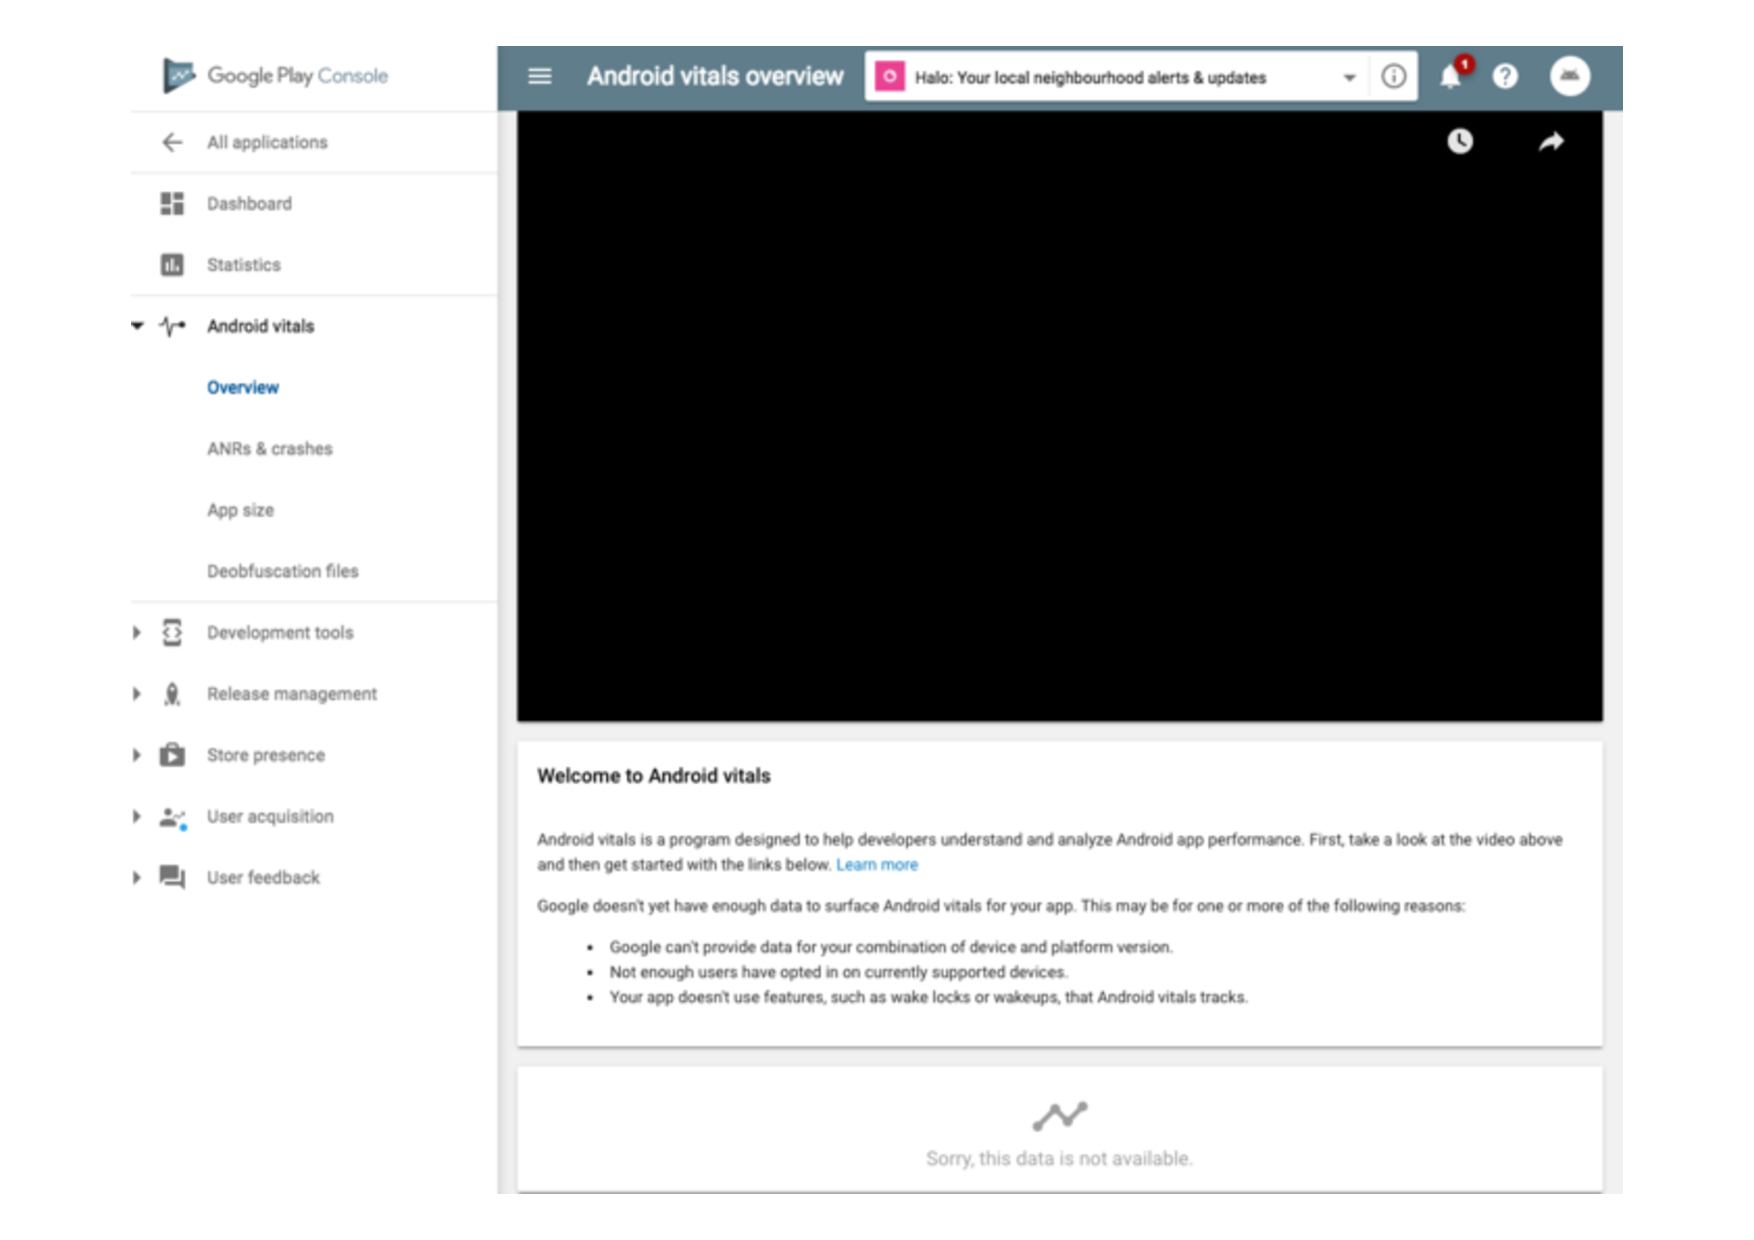
\includegraphics[width=\linewidth]{images/localhalo/apphealthoverviewplace_5550596_no_data.pdf}
  \captionof*{figure}{App Health Overview page}
\end{minipage}\hfill%
\begin{minipage}{.45\linewidth}
  \centering
  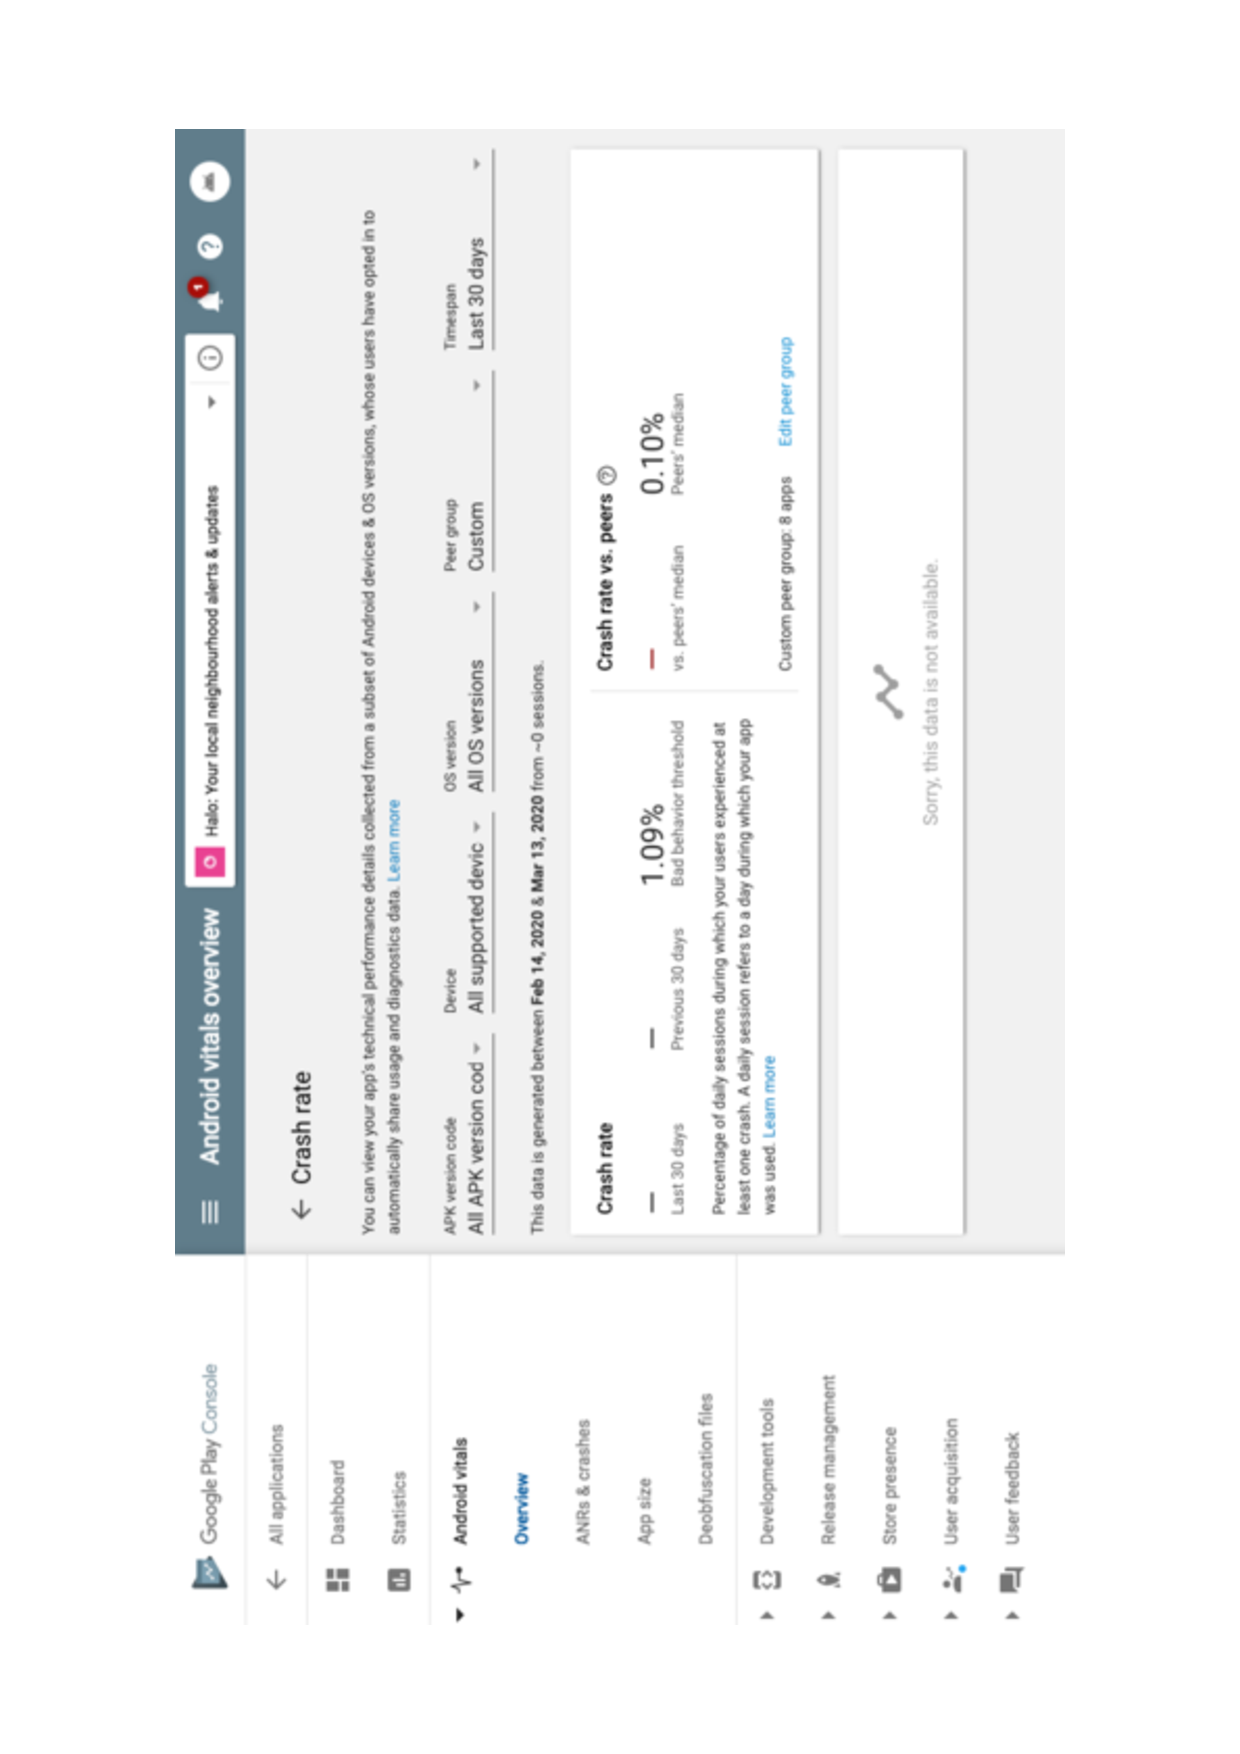
\includegraphics[width=\linewidth]{images/localhalo/apphealthdetailsplace_55505963_no_data.pdf}
  \captionof*{figure}{App Health Details page}
\end{minipage}
    \caption{No Android Vitals reports on \nth{16} March 2020}
    \label{fig:localhalo-android-vitals-no-data-16-march-2020}
\end{figure*}

Figure~\ref{fig:localhalo-android-vitals-high-failures-26-march-2020} was recorded ten days later in \nth{26} March 2020 and shows the alerts for both high crash and ANR rates in the App Health Overview page and the graph for the rampant crash rate in the corresponding App Health Details page. These indicate the failures were related to the native runtime rather than within the React Native code. These were not reported by any Sentry Alerts and they do not appear in the weekly summary reports, except potentially by the absence of data shown in Figure~\ref{fig:sentry-missing-data-march-2020}. While the reason for this was not explained in the interviews or in the analytics data, it is likely that this caused by severe crashes that prevented Sentry's SDK from reporting any data.

\begin{figure*}[htbp!]
\RawFloats
\centering
\begin{minipage}{.45\linewidth}
  \centering
  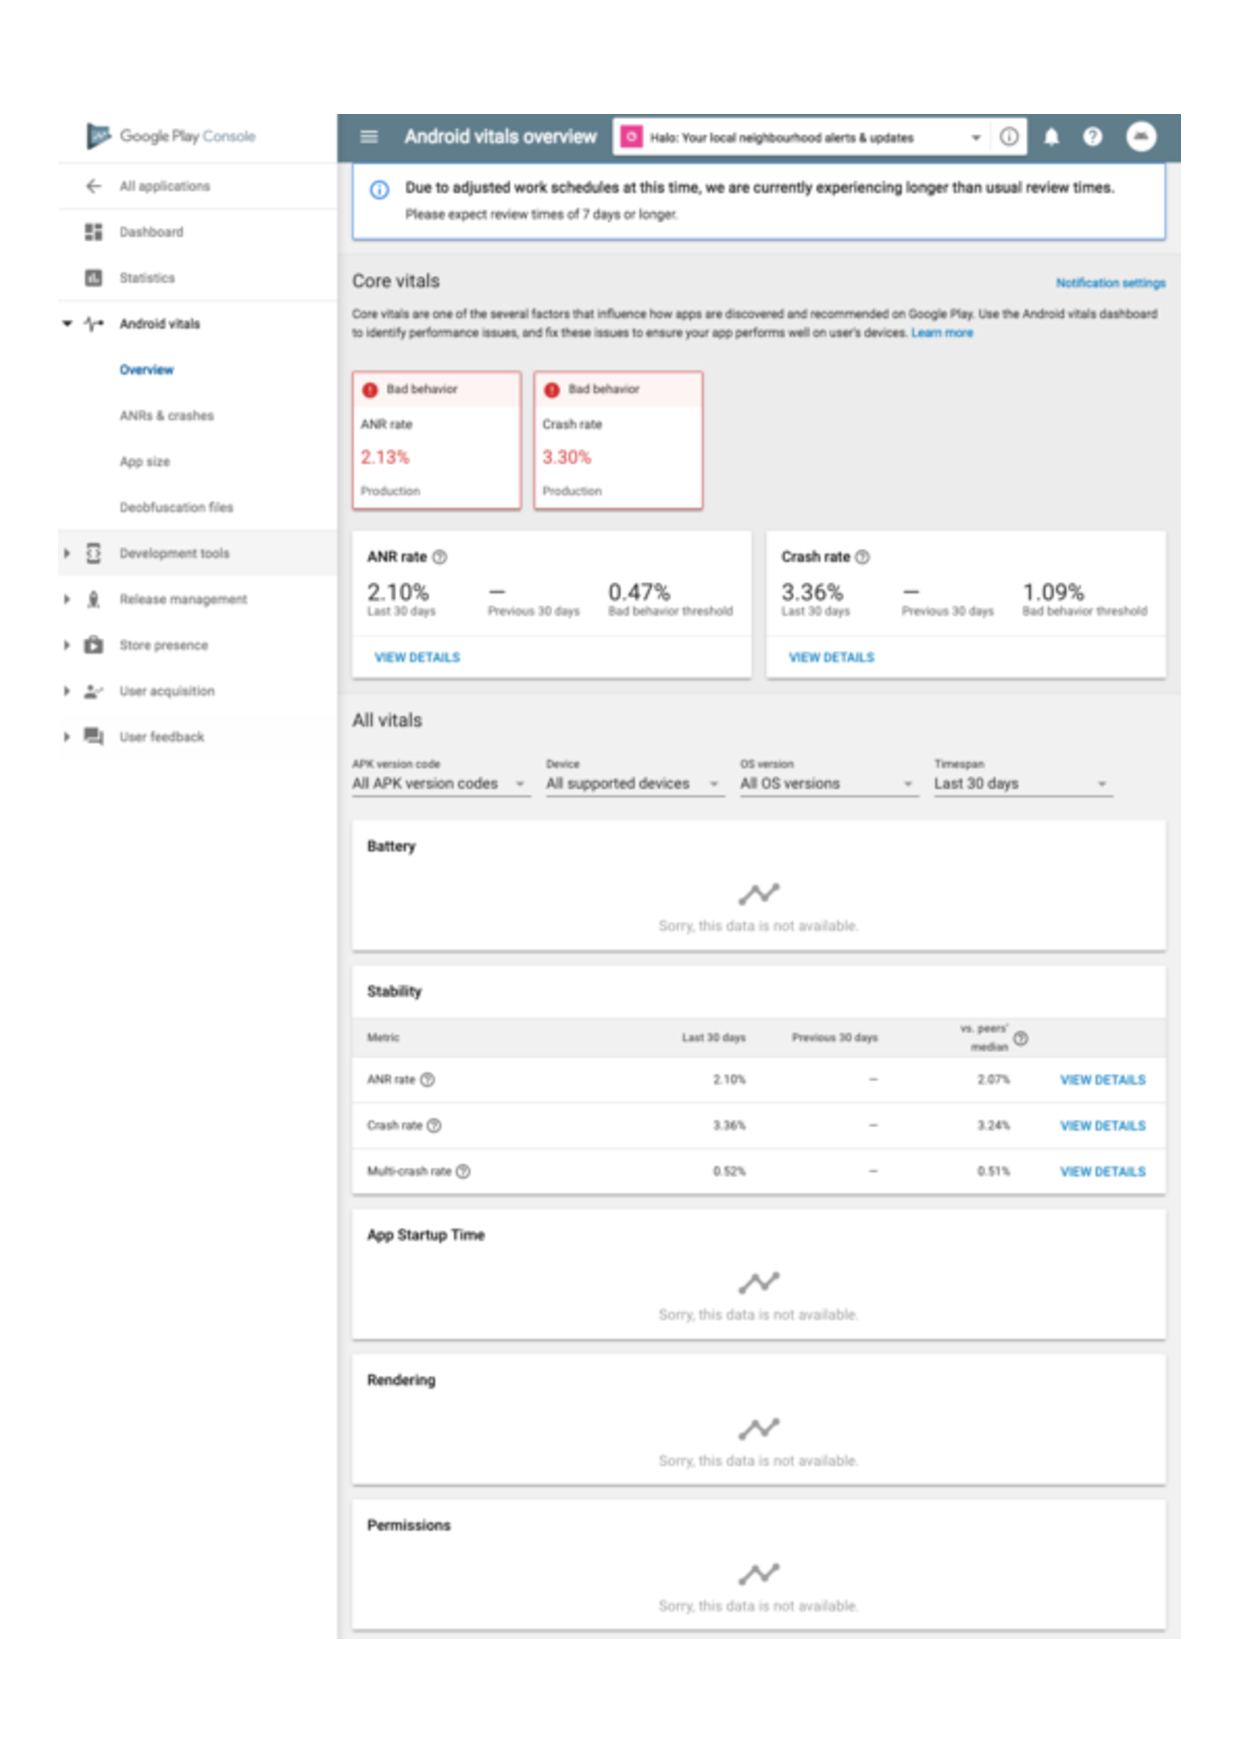
\includegraphics[width=\linewidth]{images/localhalo/apphealthoverviewplace_5550596_high_errors.pdf}
  \captionof*{figure}{App Health Overview page}
\end{minipage}\hfill%
\begin{minipage}{.45\linewidth}
  \centering
  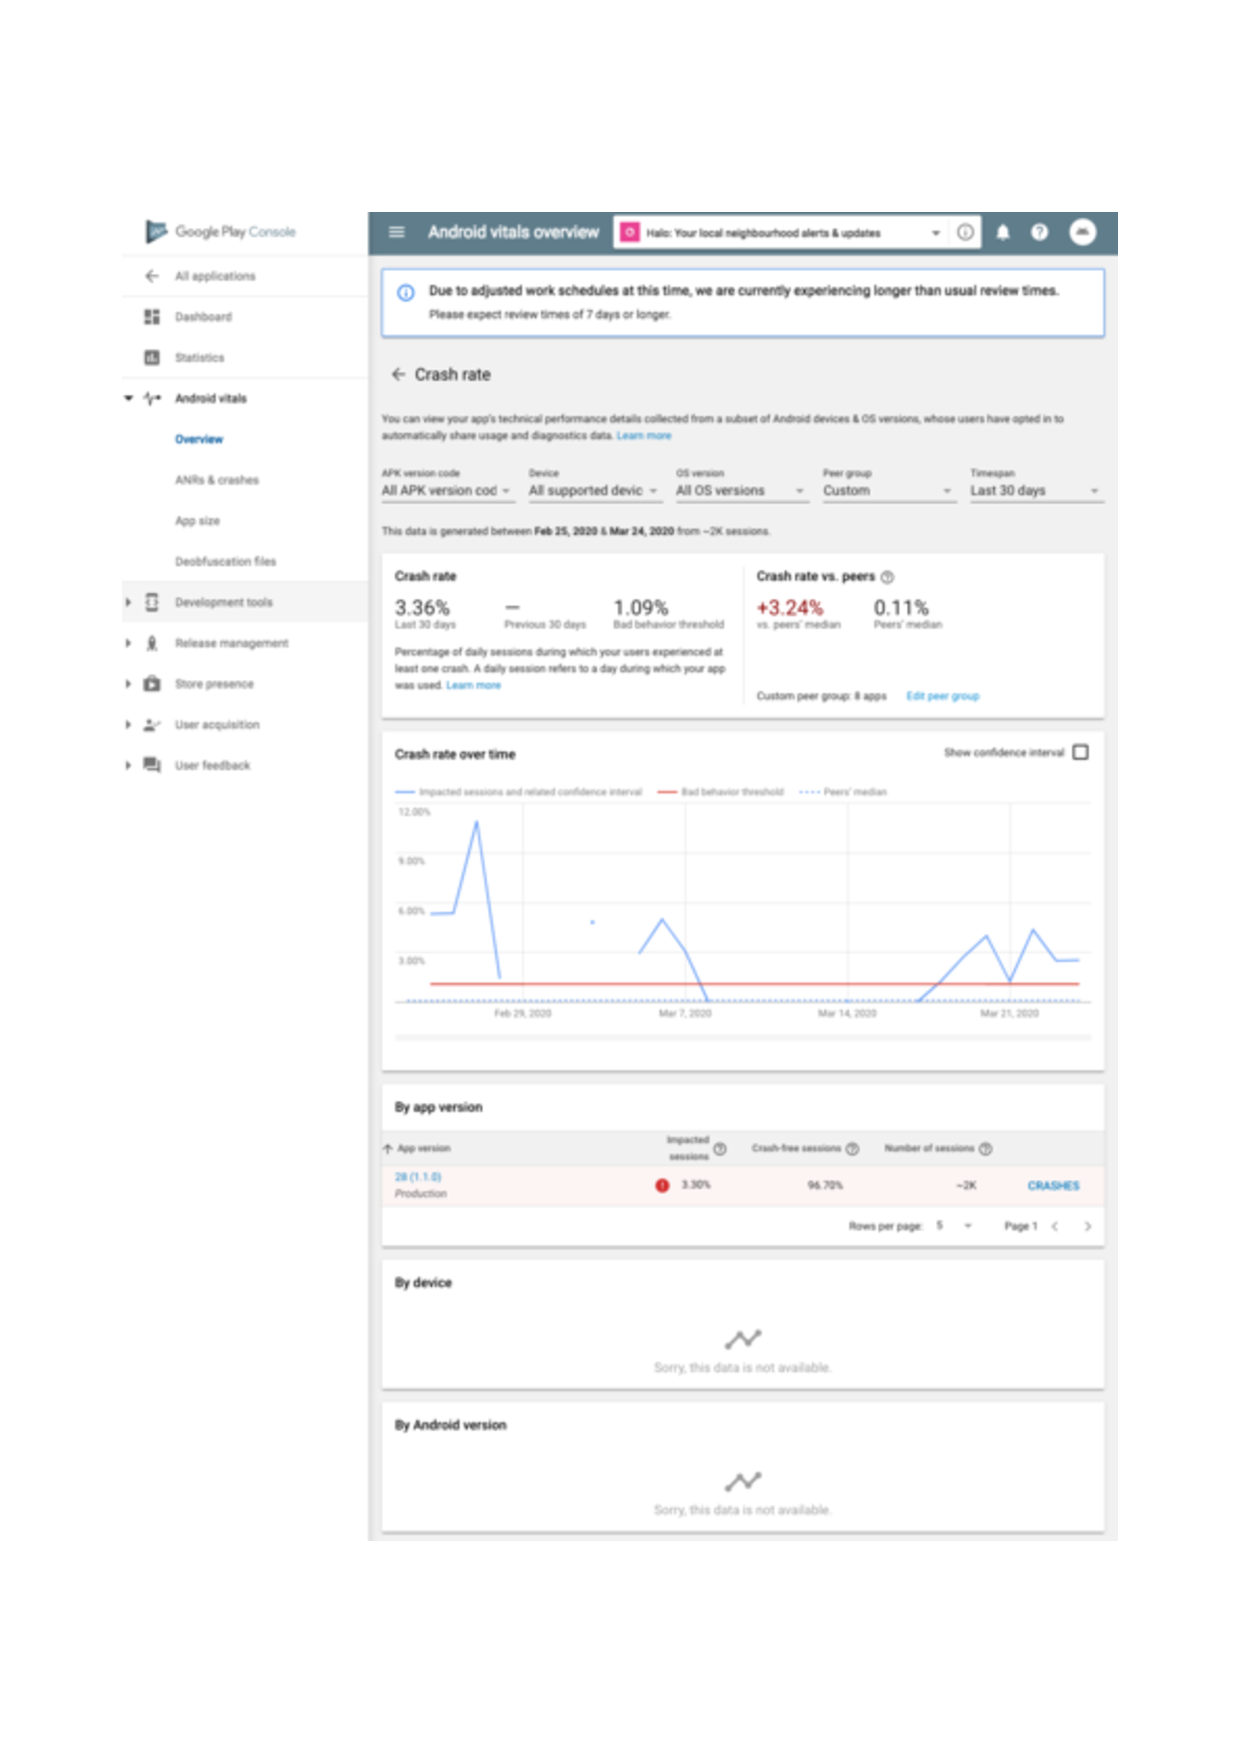
\includegraphics[width=\linewidth]{images/localhalo/apphealthdetailsplace_55505963_high_errors.pdf}
  \captionof*{figure}{App Health Details page}
\end{minipage}
    \caption{Alerts and graphs in Android Vitals on \nth{26} March 2020}
    \label{fig:localhalo-android-vitals-high-failures-26-march-2020}
\end{figure*}

A release in March 2020 had a high crash rate for the production release of their Android app. The top crash cluster was for:

{\small \texttt{java.lang.RuntimeExceptionhost.exp.exponent.experience.a\$b.run}} 

This was traced to a problem in the expo library the development team used in the app~\sidecite{expo2019_issue5839}~\footnote{Expo is a very popular open source platform for making universal native apps that run on Android, iOS, and the web \url{https://github.com/expo/expo}.}. In that issue, several developers for different Android apps provide data from Google Play Console confirming they also receive similar crash clusters. The cause has not yet been definitively traced or addressed, however for the LocalHalo app the crashes stopped being reported once a new release (1.3.0) of the Android app, was launched around \nth{6} April 2020.


\begin{figure*}[htbp!]
\RawFloats
\centering
\begin{minipage}{.45\textwidth}
  \centering
  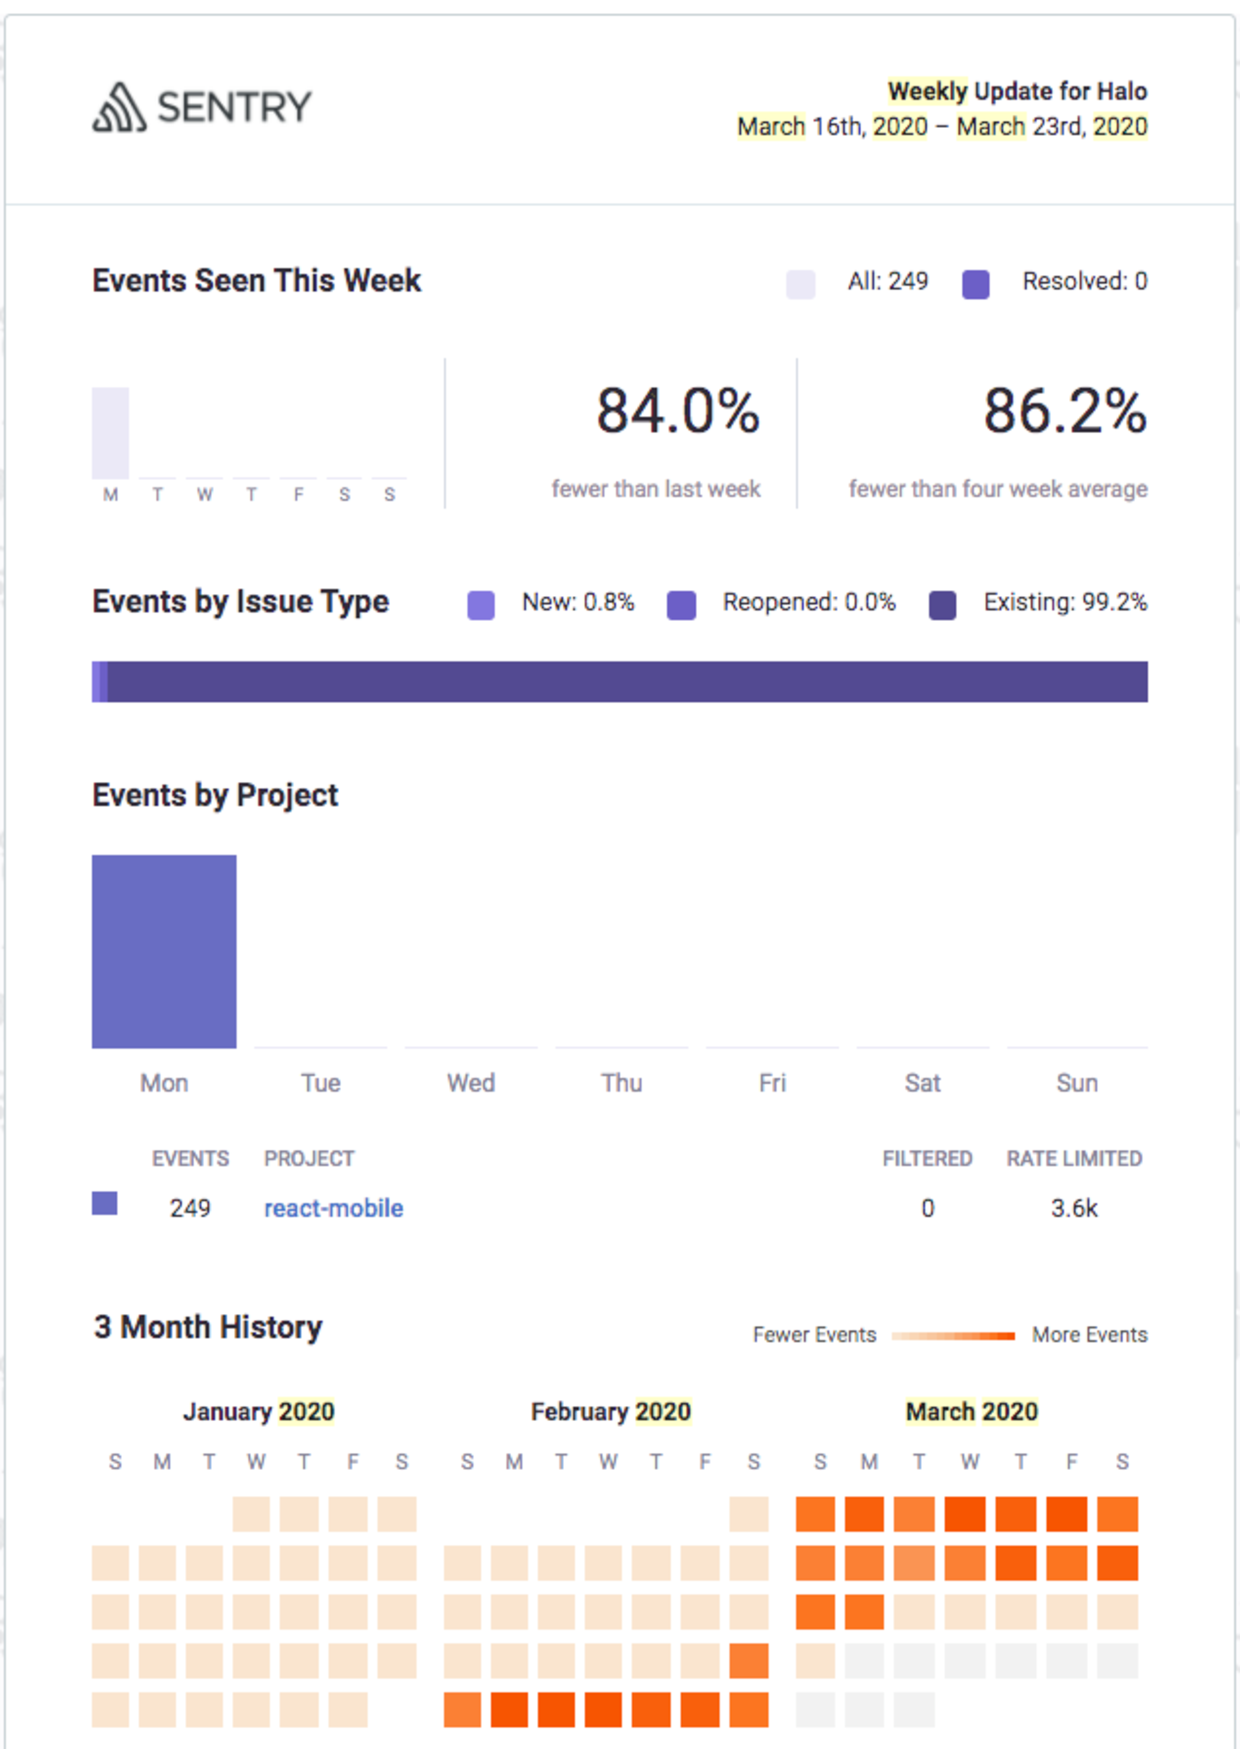
\includegraphics[width=\textwidth]{images/localhalo/sentry-weekly-report-16-mar-2020.pdf}
  \captionof*{figure}{\nth{16} -~\nth{22} March 2020}
  \label{fig:localhalo-sentry-weekly-report-16-mar-2020}
\end{minipage}\hfill%
\begin{minipage}{.45\textwidth}
  \centering
  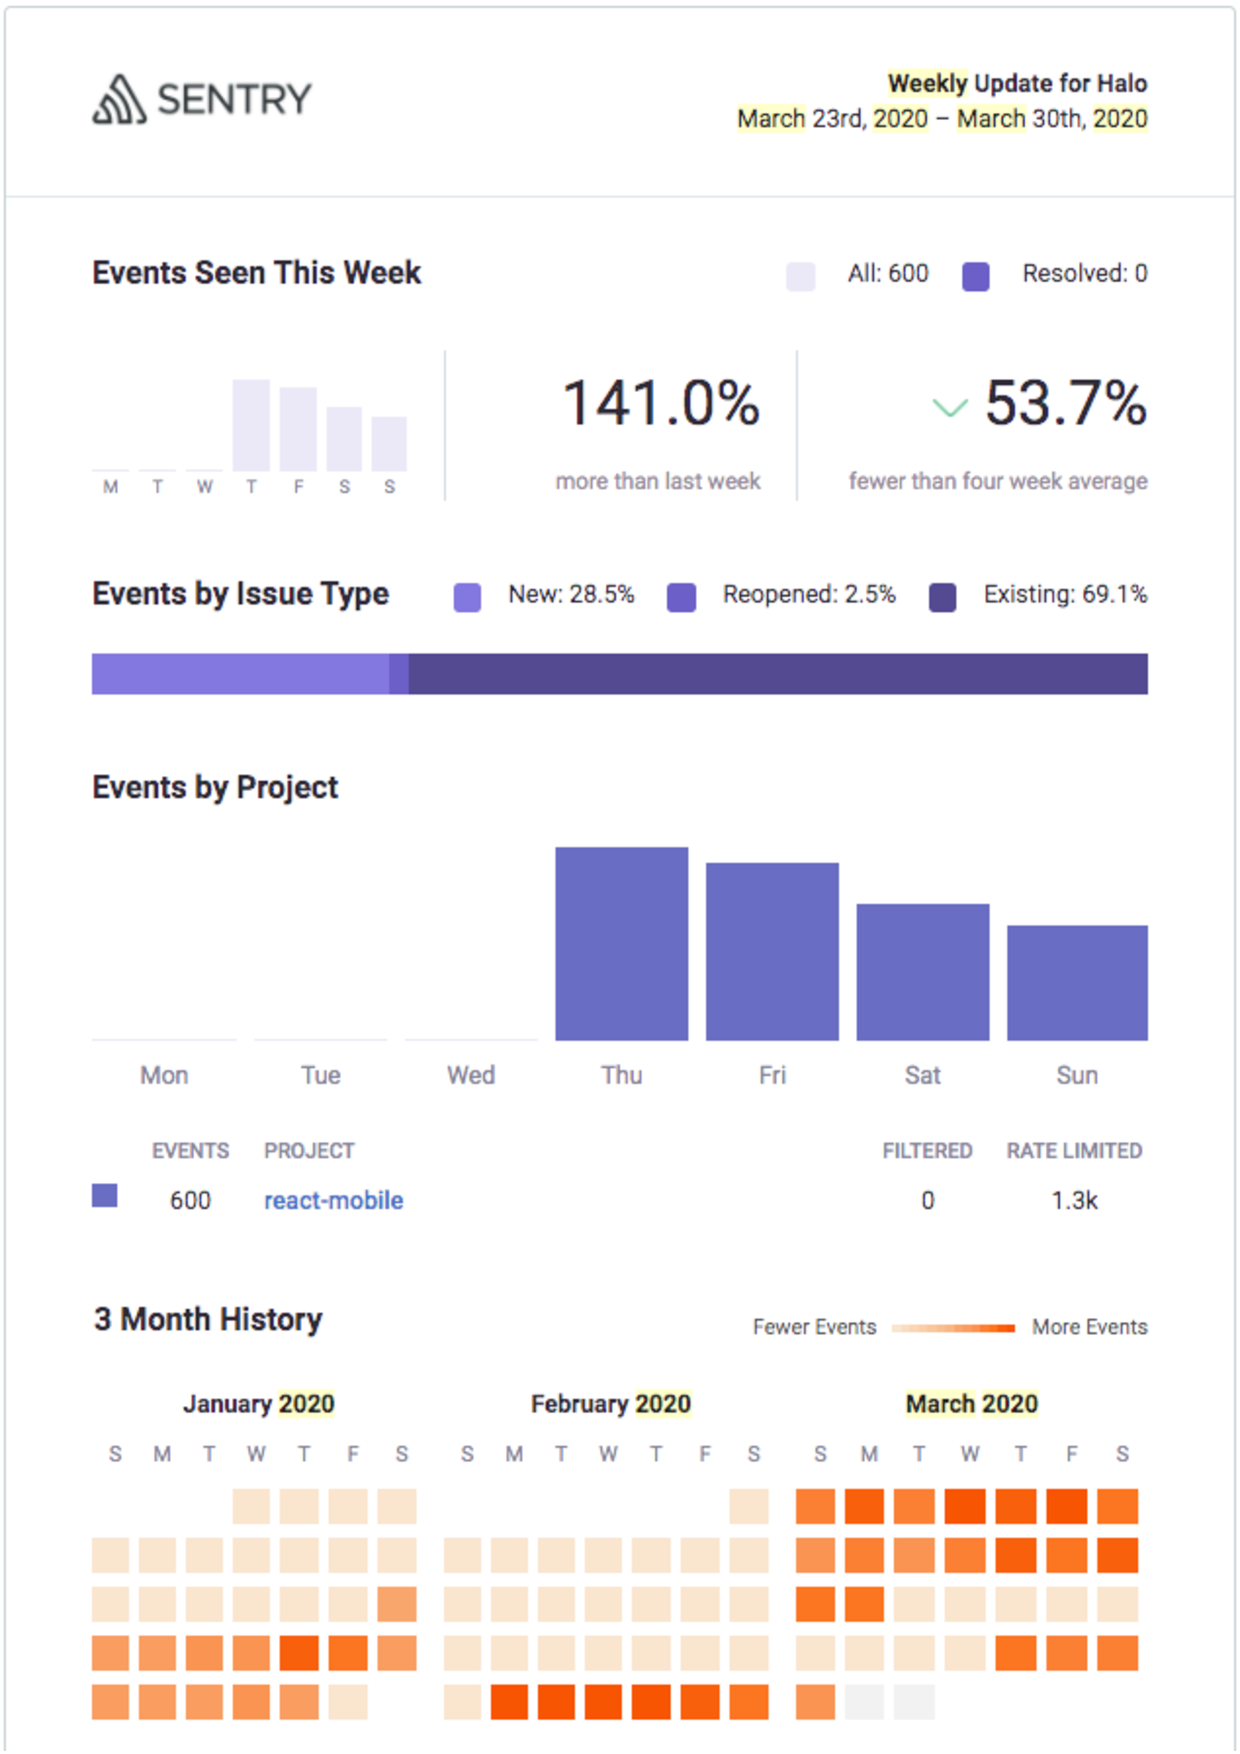
\includegraphics[width=\textwidth]{images/localhalo/sentry-weekly-report-23-mar-2020.pdf}
  \captionof*{figure}{\nth{23} -~\nth{29} March 2020}
  \label{fig:localhalo-sentry-weekly-report-23-mar-2020}
\end{minipage}
    \caption{Missing data reported in Sentry, in March 2020}
    \label{fig:sentry-missing-data-march-2020}
\end{figure*}

\newthought{Some failures did emerge when the runtime encapsulation fails: }
That exception was when Android Vitals did report crashes in March and April 2020. Figure \ref{fig:localhalo-android-vitals-no-data-16-march-2020} was recorded on \nth{16} March 2020 before these started and shows the App Health Overview page with a link to a video introducing Android Vitals~\sidenote{This appears as a mainly black rectangle in this thumbnail screenshot.}, and the App Health Details page with no data.

\subsubsection{Meta-data}~\label{section-meta-data}
Meta-data is not about the app \emph{per se}, but about the user and/or the user's device, \emph{etc.} 
Meta-data may help developers with bug localisation and reproduction pertaining to the device model, its underlying hardware characteristics, the release of the platform, and so on. 

Figure \ref{fig:fabric-crashlytics-privacy-policy} provides an illustration of the privacy policy for Fabric Crashlytics which lists various the meta-data it collected at the time. The successor Firebase Crashlytics lists similar data being collected for crashes~\url{https://firebase.google.com/support/privacy#crash-stored-info}. The details of why these details were necessary was discussed online by \href{https://stackoverflow.com/users/3975963/mike-bonnell}{Mike Bonnell}, 
one of the Crashlytics engineering team, in response to a question on StackOverflow~\sidecite{kim2017_what_information_does_crashlytics_collect_from_end_users}.

\begin{figure}
    \centering
    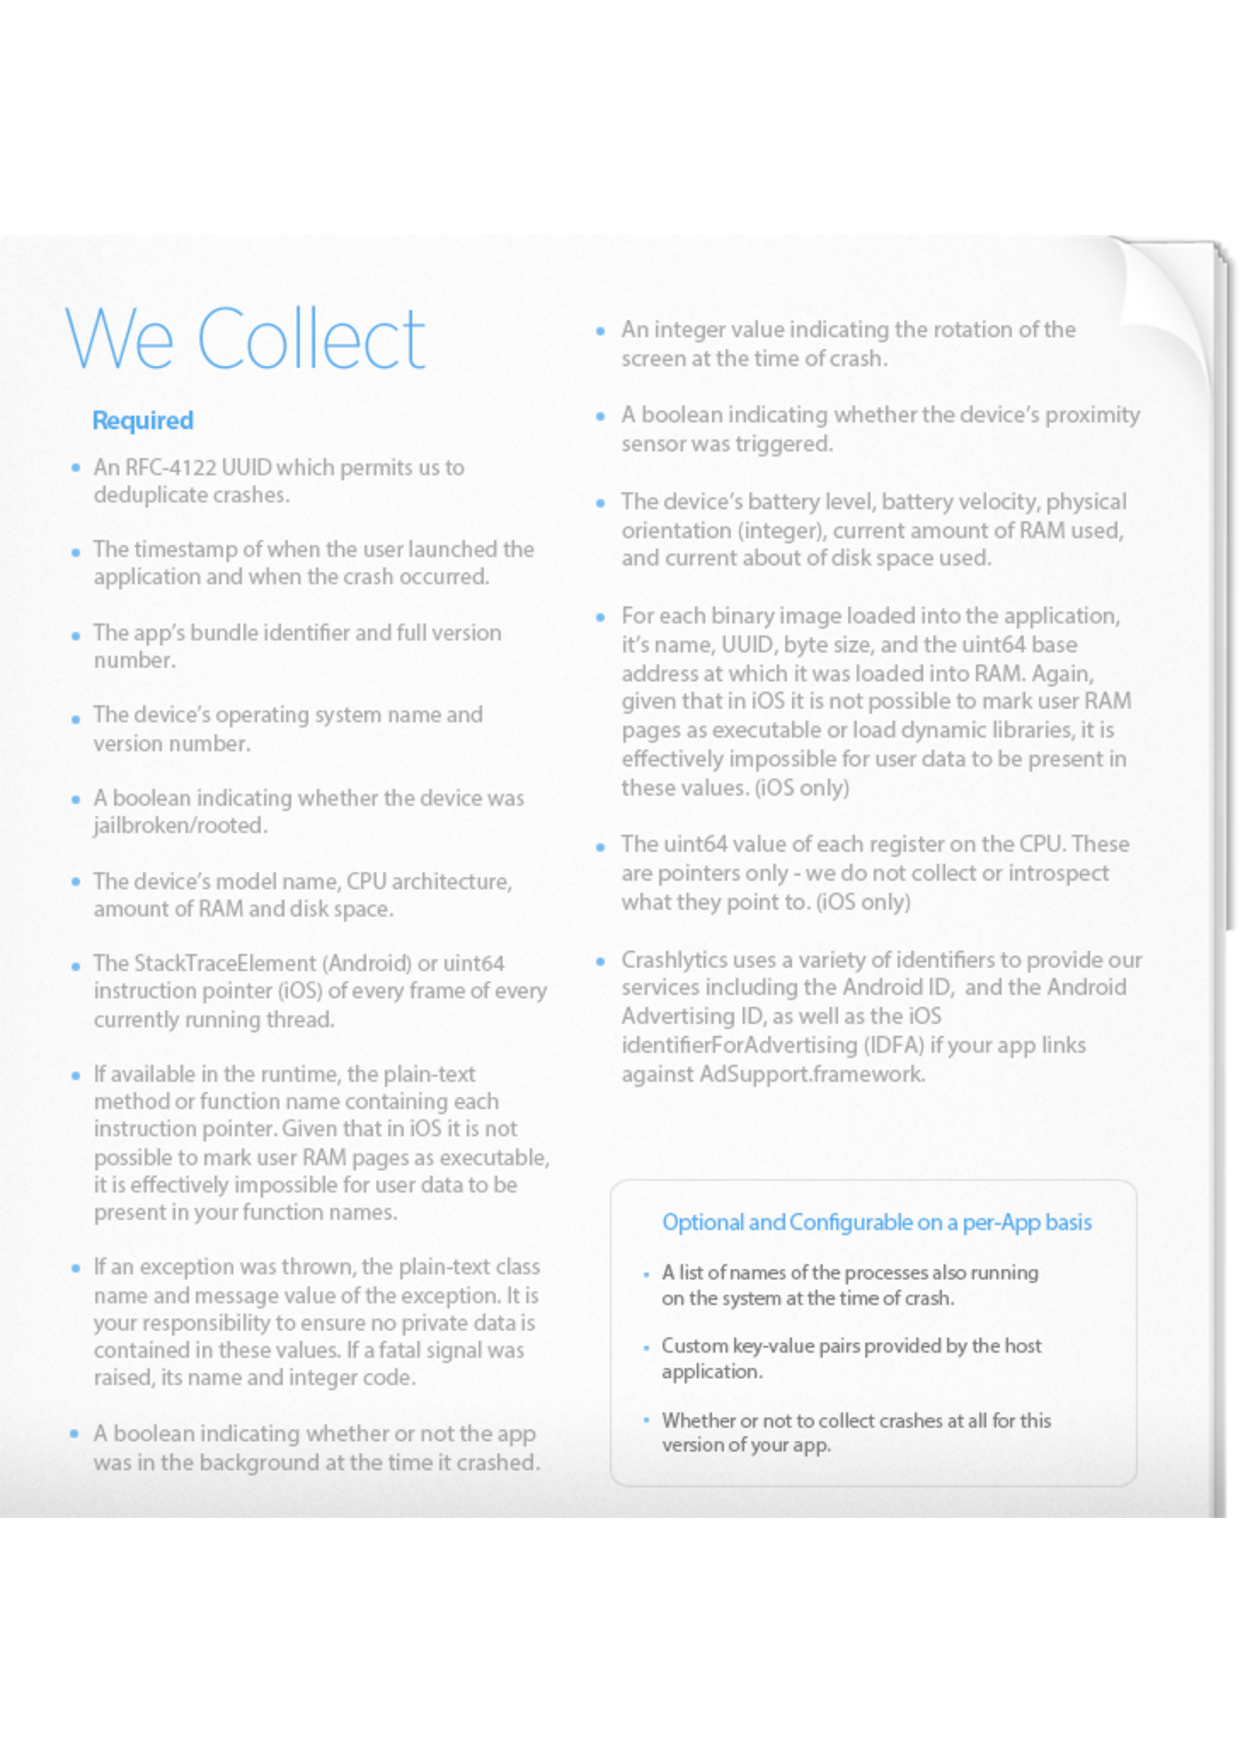
\includegraphics[width=10cm]{images/fabric-crashlytics/crashlytics-privacy-policy-38154ffbd69ef44a478b54365dc9b3ad.pdf}
    \caption[Fabric Crashlytics Privacy Policy (in 2015)]{Fabric Crashlytics Privacy Policy (in 2015)\\{source: \tiny \url{https://web.archive.org/web/20150405071731/http://try.crashlytics.com/security/}}}
    \label{fig:fabric-crashlytics-privacy-policy}
\end{figure}

Of note, some app developers may receive data they didn't expect, particularly if they migrated from \myindex{Fabric Crashlytics} to \myindex{Firebase Crashlytics}. 

To provide some additional context Fabric and Firebase both offered facilities to combine various datasets into their reporting, for instance based on advertising SDKs. This led to reports that included demographics in addition to the crash analytics, \emph{etc.}~\footnote{Discussions on how the demographics are captured and made available include~\cite{joe2016_firebase_analytics_demographics} and~\cite{chelo2020_firebase_does_not_collect_age_or_gender_data}.}. 

The forced migration from Fabric Crashlytics to Firebase Crashlytics had two stages, the first was to migrate the project to the Firebase user interface and the second was to replace the Fabric SDK with the Firebase SDK. The Firebase SDK automatically collected additional data~\sidecite{firebase_help_GA4_2021_predefined_user_dimensions}.


As mentioned in \secref{aata-tradeoffs-topic}, the Catrobat project chose to stop using Firebase Crashlytics when they discovered that the demographics of the end users were also being recorded. 

In collaborative research into using Firebase Analytics for logging, 50 of 107 active Android opensource projects initialised just the Firebase Analytics SDK; they did not use any other aspect of the SDK~\sidecite{harty2021_logging_practices_with_mobile_analytics}~\sidenote{Perhaps they thought that `Getting Started' was all they needed to do? or perhaps the default data was `good enough'?}. Therefore the contents and the limitations of the default meta-data are of particular interest, since default meta-data is all those developers would have available to them. The remaining 57 projects used additional API calls to record additional information on one or more code-paths in the respective app.

\subsubsection{Engineering challenges}~\label{section-engineering-challenges}
Engineering challenges relate to developing the components of the mobile analytics tool/service such as provision of a client-side SDK that collects failures for native (C++) code.

Engineering challenges for mobile analytics include:
\begin{itemize}
    \item Support for collecting information from native code. This can be particularly pertinent for apps that include libraries in native code that are provided by third-parties.
    \item Collecting information from the earliest stage of app startup to the app's shutdown; otherwise data collection is incomplete.
    \item Establishing and maintaining sufficient information to calculate and provide sufficiently accurate comparisons, ratios, and so on. As an example, determining the Probability of Failure On Demand (\href{glossary-pfod}{PFOD}), requires counts of non-failures -- those events/transactions/\emph{etc.} that \emph{worked}. Also, the sources/inputs/conditions that contributed to the failure may be useful to the app developer; does the mobile analytics SDK collect these? In the \myindex{Kiwix} case study; there were various sources of WebView crashes, these needed to be identified in order to attempt to prevent similar crashes in future.
    \item For the Vitals Scraper utility developed as part of this research, there were engineering challenges in first developing and then maintaining an automated interface to obtain reports and related information from Google Play Console and Android Vitals.
    \item For platform tools, collecting pertinent information across the process boundary includes engineering challenges. For in-app analytics, collecting information, such as ANRs, was a challenge during the period of the active app-centric case studies. 
\end{itemize}

These challenges are ongoing, various \Glspl{sdk} aim to address one or more of them.

\subsection{Developer experience}~\label{tata-developer-experience-ux-design}
The design of the User Experience (UX) of the mobile analytics tool for their audience of the software development team (and particularly the app developers).

% TODO add examples from the case-studies

\newthought{Vying for the attention of developers: }
Mobile Analytics tools compete for finite attention developers are able to provide. This competition occurs at the initial selection and integration phases and continues during the life of the app. This includes seeing attention on an ongoing basis  to communicate their alerts, reports, \emph{etc.} Pricing, licensing, and management approvals sometimes prevent some development team members from being able to use the tools directly.

\begin{itemize}
    \itemsep0em
    \item Access and use of mobile analytics tools allows them to be used interactively, where this is impractical copies, extracts, \emph{etc.} of reports and related material helps  preserve them for future analysis, for evidence, and so on. These copies and extracts can also extend the reach to people who don't have direct access to the tools. Several of the app-centric case studies, including Kiwix, Catrobat, LocalHalo, and the Commercial project limited access to various tools to a subset of the developers. In contrast, Moonpig, provided access to every member of the development team who had access to the source code of the app.
    \item When the analytics tools lack the attention of developers the effects of existing and new issues propagate and may enable these issues to snowball. The Kiwix project provided a good example of this with the loss of the lead developer for the Android app.
    \item The majority of the app-centric case studies used multiple mobile analytic tools. Some of the developers chose to ignore aspects of particular tools, for instance the crash analytics in Android Vitals in favour for similar services from other tools, even though Android Vitals is able to record some crashes that the other tools do not capture \emph{e.g.} owing to limitations in the respective SDK. The tools need to convince developers of the merits of their reports. The Moonpig development team, in particular, checked the reports of multiple tools to reduce their blind-spots.
    \item The LocalHalo project illustrated the flip-flop of failures between two analytics tools. This was insightful and demonstrates the value of having a combination of platform-level and in-app analytics, at least for apps written in frameworks such as react-native.
\end{itemize}


\section{Fitness-for-purpose}~\label{tata-fitness-for-purpose-section}
Simply put, the mobile analytics tools need to be fit for purpose. In the context of this research, fit for purpose means that the tools need to:\todo{Revisit the following list once I've added the subsections.}

\begin{itemize}
\item fit the needs and desires of the developers (product fit); 
\item provide actionable reports; and 
\item be a good return on any investment the developers make in terms of using the tools.
\end{itemize}
 
When the tools integrate into the workflows of the developers, they're more likely to be adopted as long-term companions and therefore demonstrate they provide a good return on investment. 

Note: two of the topics: fidelity and ethical considerations bridge both this section: fitness-for-purpose and the dependability section.

{\small
\begin{itemize}
    \itemsep0em
    \item \sout{Product Fit: whether, and if practical how well, the mobile analytics product fits the desires/needs of the developers and their organisation.}
    \item \sout{Actionable Reports: reports the developers can action in order to address concerns presented in the reports.}
    \item \sout{Integration into workflows: the ability of a given mobile analytics tool/service to be integrated into development team's workflows.}
    \item Ethical considerations: the data collected by mobile analytics may have ethical implications a) for the operator/provider of the service, b) for their partners and customers, c) for the developers, d) for end-users. In this research our main focus is on the implications for the developers, nonetheless the other aspects are also important.
    \item ROI (return-on-investment): developers may make both implicit and explicit choices on what to invest in, for instance in terms of their focus, their effort, and their money. The analytics tools need to convince developers a) to invest and then b) whether to increase that investment (and if so what forms of investment e.g. in terms of writing more code, spending [more] money, using the tool more, etc.).
\end{itemize}
}

\subsection{Product Fit}
\newthought{Product fit: } addresses whether, and if practical how well, the mobile analytics product fits the desires/needs of the developers and their organisation. It is similar, but more specific than product/market fit~\footnote{\url{https://en.wikipedia.org/wiki/Product/market_fit}} - or conversely the market is pico-sized, gauged at the level of a development team. % See also concepts from https://en.wikipedia.org/wiki/Lean_startup e.g. actionable metrics.

Developers of mobile analytics tools, such as Iteratively~\sidenote{Iteratively was acquired by Amplitude in 2021 and the products have been enhanced and integrated into Amplitude's product suite.}, seek ways to identify and determine what app developers will find useful. 

In interviews with Iteratively's CEO, he explained they used various techniques including `ten dots', illustrated in Figure \ref{fig:iteratively-product-market-fit}, during one-to-one semi-structured interviews to help Iteratively prioritise the features they developed and provided. Each interviewee was given the opportunity to complete this exercise, an example of their `dot-voting'~\sidecite{18f_dot_voting} is also provided in Figure \ref{fig:iteratively-product-market-fit}.
The CEO provided access to their live document containing the results of the `dot-voting' and gave permission to analyse it.~\todo{Consider whether to include the analysis of the dot-votes (currently in the relevant empirical studies chapter).}


\begin{figure}[htbp!]
\RawFloats
\centering
\begin{minipage}{.45\textwidth}
  \centering
  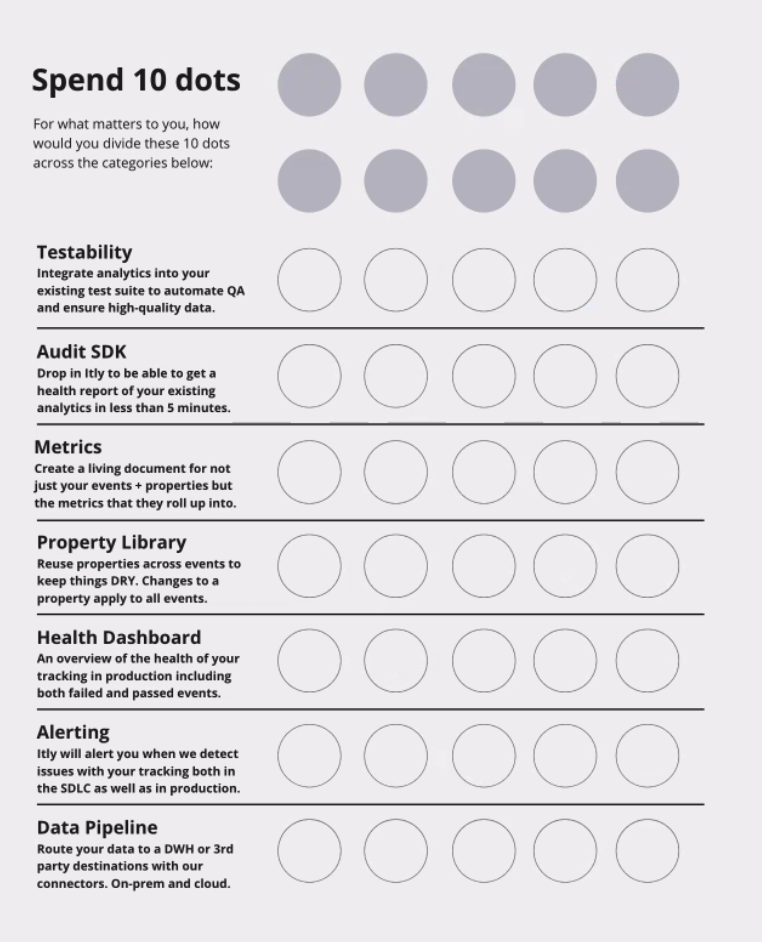
\includegraphics[width=\textwidth]{images/iteratively/spend-10-dots.png}
  \captionof*{figure}{Spend ten dots}
  \label{fig:iteratively-spend-ten-dots}
\end{minipage}\hfill%
\begin{minipage}{.45\textwidth}
  \centering
  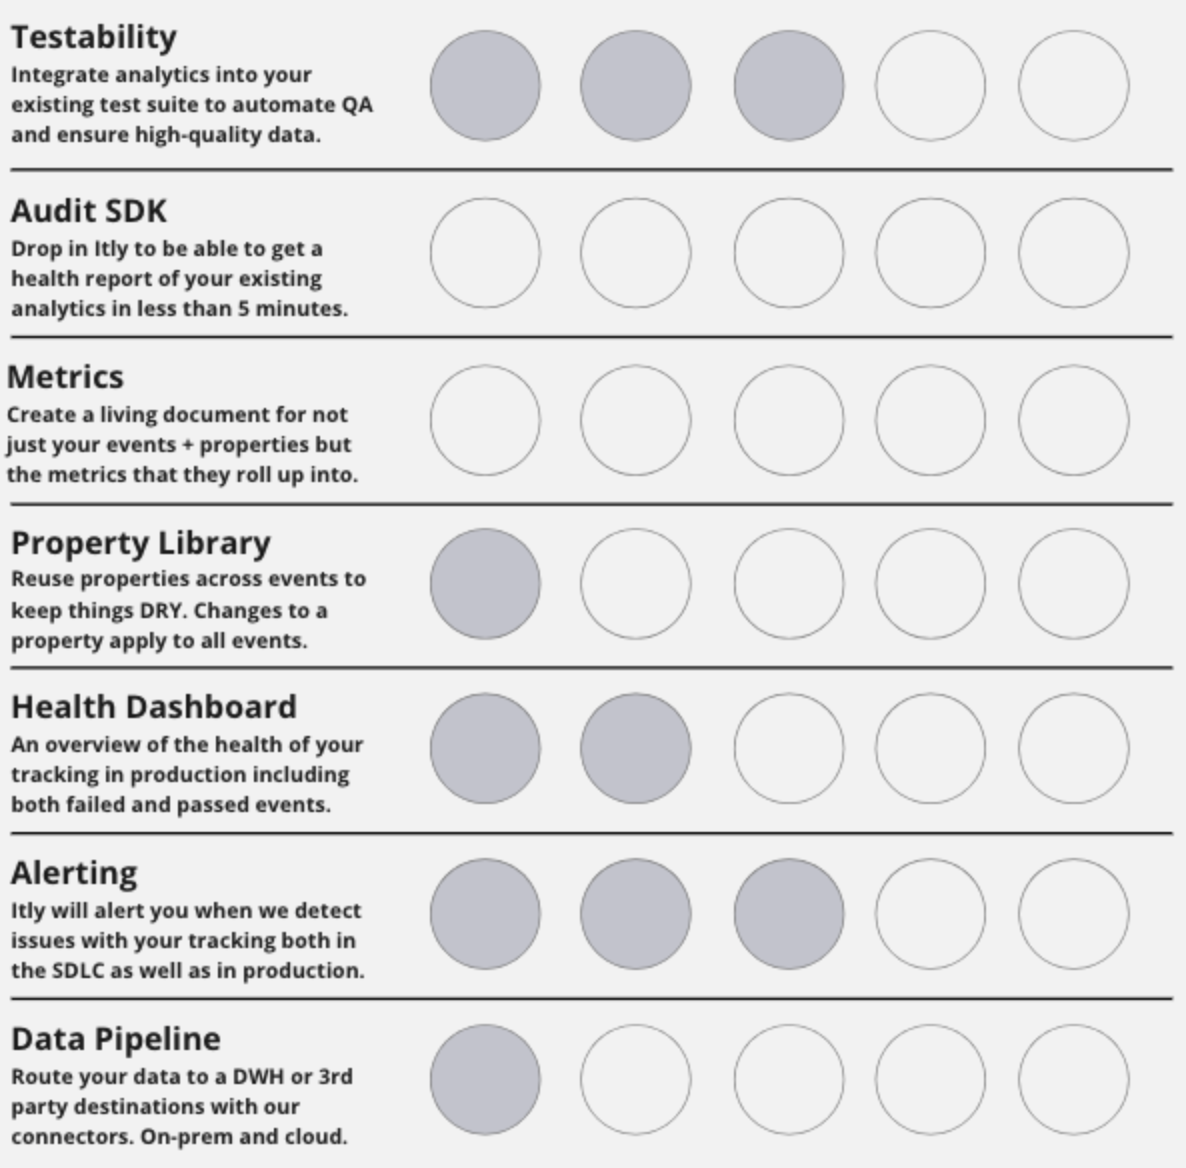
\includegraphics[width=\textwidth]{images/iteratively/dot-voting-example.png}
  \captionof*{figure}{Dot-voting example}
  \label{fig:iteratively-dot-voting-example}
\end{minipage}
    \caption{Iteratively: Product/Market fit}
    \label{fig:iteratively-product-market-fit}
\end{figure}

\myindex{Iteratively} had developed a combination of an online design tool that created a schema for third-party in-app analytics tools. They also provided build tools and a small client-side SDK (\textit{i.e.} a mobile \Gls{sdk}) which validated the schema had been implemented adequately in the mobile app. %, where all the data from the schema and only the data from the schema would be collected by the relevant mobile analytics SDK.
Iteratively's SDK was intended to limit the collection to only the data contained in the schema. This was intended to stop the collection of other data (such as \Gls{pii} data). Through the use of the SDK, the build tools, and the online design tool development teams and their colleagues with other roles such as marketing, product, and so on could have a consistent and coherent understanding of the data that was being collected. Of interest to this research, they did not address the collection of errors or failures such as crashes in their SDK.

\myindex{LocalHalo} are a good example of a small development team who chose to include several mobile analytics SDKs into their mobile app where each SDK (and the respective service) was chosen to provide orthogonal data. They chose \href{https://sentry.io/}{Sentry} for technology facing analytics and \href{https://mixpanel.com/}{mixpanel} for product (business facing) analytics. Although Sentry provides APIs~\footnote{\url{https://docs.sentry.io/api/}} for integration and data forwarding~\footnote{\url{https://docs.sentry.io/product/data-management-settings/data-forwarding/}} and mixpanel provides data pipelines~\sidenote{\url{https://mixpanel.com/data-integrations/}} LocalHalo did not use these. In contrast for the large commercial project data integration was deemed vital by the organisation in order to facilitate ongoing and \emph{ad-hoc} analysis across multiple sources of information. 

In the case of the corporate project, \myindex{C1}, the product (the mobile analytics tool) also had to fit at the level of the engineering organisation where the mobile analytics needed to be ingested into the corporation's `data-lake'. 

Finally for this topic, despite many mobile analytics SDKs, there may be situations where none provides the answers the developers seek. As a concrete example, \myindex{Smartnavi} uses \myindex{Firebase} and \myindex{Google Analytics}, mainly for tracking the popularity and the use of the app's features. The app also incorporated Fabric Crashlytics for crash reporting. Nonetheless the developer explained none of these analytics products provided analytics related to software running in the background, as a background process on Android. Smartnavi provides GPS services to other apps and runs in the background. As the Android Platform has evolved Google has embedded restrictions that limit and constrain background processes which meant the Smartnavi software is suspended (paused) by Android. The developer would like to improve the app's behaviours when it runs in the background but lacks the analytics to do so.

\subsection{Actionable Reports}
\textbf{Actionable Reports} are reports the developers can use to decide on what should be done to address concerns presented in the reports. % c.f. actionable metrics https://effectivesoftwaredesign.com/2021/03/23/lean-startup-principles-vanity-metrics-and-actionable-metrics/

Several of the app-centric case studies materialised because the respective development teams became aware of excessive and chronic error rates for their mobile apps. % Kiwix, Catrobat, C1
These projects (\myindex{Kiwix}, \myindex{Catrobat} and \myindex{C1}) had not managed to materially reduce the high crash rates directly and they were happy to receive help and insight in how to apply the information from the reports in their work. At the time they lacked the wherewithal to do so unaided. With interventions, including those that were part of this research, each of the development teams were able to materially improve the error rates of their respective apps.

None of the currently available mobile analytics tools seen during this research were able to pinpoint the causes of failures, instead they identify one or more effects \emph{e.g.} the app crashes, or is stopped by Android because it became unresponsive. The action-ability comes in part from the meta-data collected by the various mobile analytics tools which helped in bug localisation and in part from the characteristics and patterns contained in the reports. The Moonpig developers, for example, were sometimes able to identify a highly likely reason for the failure from the contents in the reports. They took action by modifying the application's source code.

\myindex{Android Vitals} aims to highlight emerging problems with a deployed app. For instance if there is an acute and significant increase in the crash rate for the production release(s). It also provides cross-connections between problems found in Google Play's pre-launch reports and failures that occur in production. Developers found some of the reported failures easy to comprehend and address, others have been much less tractable. Several of the developers who use Crashlytics said they preferred using it over Android Vitals for comprehending crashes. \myindex{Crashlytics} provided more information than Android Vitals and the reports were easier to digest therefore the Crashlytics reports were more actionable than those from Android Vitals.

As discussed in the flaws topic (\secref{section-flaws-in-the-analytics}, \secref{section-flaws}) various reports have flaws, for instance in their aggregation. There is scope to improve the mobile analytics tools through improving the matching process in the data aggregation (for instance, where there are fragmented `failure clusters') and in the analysis across multiple legitimate failure clusters (such as across all \texttt{NullPointerExceptions}) to help identify underlying flaws in the development of the app.

The \myindex{Moonpig} case study provides an illustrative example of how the development team was able to take proportionate and measured action as the crash-rate of their Android app increased. The cause was related to a known and documented issue with a third-party software library, RoboSpice. There was a clear correlation where the crash-rate increased on newer Android releases. The team was able to evaluate and estimate an appropriate timescale to replace that library by revising the application's source code. They were able to schedule the release to suit other strategic objectives rather than rushing to push out a `fix' of the app.

The release management reports in Google Play Console (that incorporate various Android Vitals reports pertinent to the latest release for the 7 days post release) were highly actionable for the Commercial project. The development team were able to abort releases that had unexpected increases in failure rates before those flawed releases adversely affected swathes of the userbase.

\subsection{Integration into workflows}~\label{tata-integration-into-workflows-section}
Integration into workflows is the ability of a given mobile analytics tool/service to be integrated into development team's workflows. These workflows include bug tracking and release management. Some mobile analytics tools provide facilities where developers can mark and/or annotate elements in the reports, for instance to remove a crash cluster from the main report or to provide a bug-tracking link to help the developers streamline their work when using mobile analytics.

The\todo{Possibly move the following 3 paragraphs to the analytics in use chapter as I'm discussing what the teams did.} 
majority~\sidenote{Moodspace and LocalHalo did not provide any details of their bug tracking processes.} of the app-centric case studies partly integrated mobile analytics reports into their bug tracking process by storing at least some of the contents of the reports some of the time.  
Of the projects that recorded the failures found by mobile analytics, it appears the Catrobat project used the crash's stack trace without anything else of the crash cluster's details or analytics~\sidenote{Examples include: \href{https://jira.catrob.at/browse/CATROID-1025}{Issue CATROID-1025} and \href{https://jira.catrob.at/browse/CATROID-1030}{Issue CATROID-1030}.} Moonpig stated they recorded many of the failures however sometimes they short-circuited the bug tracking system and modified the source code directly where the likely fix was believed to be easy to address with minimal risk. As they monitored the various mobile analytics services assiduously post-release they had at least one safety-net, also they may have recorded pertinent information in their source code repository - as this was not available during the research it is impractical to check at this stage.

\myindex{Kiwix}, \myindex{Catrobat}, \myindex{LocalHalo}, only provided a subset of the development team access to the mobile analytics services. As a result, the rest of the team were blind to any reports or issues \emph{unless someone who has access provides the relevant information in the bug tracking system}. The \myindex{GTAF} project team record crashes reported by Firebase in their bug tracking system however they only embed the URL, they have not included copies of the pertinent details.



\section{\itools}~\label{tata-itools-section}


\section{Fieldstones}
\julian{These need integrating or removing pre-submission.}

An interesting phenomenon observed during the Catrobat hackathon where some of the crashes that appeared in Android Vitals were believed to come from `soft errors' in the Pocket Code app. The issue, CATROID-426, was logged during the hackathon~\sidecite{catroid_426_soft_crashes_should_not_be_reported_to_the_play_console} and the developers wrote two sets of code changes (also known as `commits'). These were merged into the app's codebase on \nth{21} Nov 2019 and released in the Pocket Code app several weeks later.

The intent was laudable, however, at least some of the soft crashes continued to occur over a month later, as documented in \url{https://jira.catrob.at/browse/CATROID-422}. This issue was raised in the hackathon and closed as a duplicate by one of the developers involved in trying to stop the soft errors from appearing in Android Vitals \sidecite{catroid_426_soft_crashes_should_not_be_reported_to_the_play_console}.

TODO Mention the Pocket Code experience when migrating from Fabric to Firebase and the additional, unexpected analytics that appeared. Forward reference to the discussion on intrusiveness.

\itools \myindex{iTools} simple facilities such as the ability to search through the failures to find any failure clusters that match. A recent example is searching for instances of an \texttt{IndexOutOfBoundsException} in the \myindex{Kiwix} custom apps\sidenote{\href{https://github.com/kiwix/kiwix-android/issues/2542}{Index Out of Bounds Exception on Custom App \#2542}} where \myindex{Android Vitals} had to be checked page by page for each app to see if the crash was still happening.

Aggregation and mining across the matching clusters would also be useful. Tagging/labelling might also help, \emph{ditto} facilities to cross-reference within and across systems (\emph{c.f.} hyperlinking and reference links.

A placeholder until the relevant content is added to check the formatting in the index for: Android Vitals\index{GitHub Projects!Android Vitals}

Breadcrumbs: in AppPulse Mobile iOS which provided similar capabilities in Android~\sidecite{microfocus2018_apppulse_mobile_android_getting_started_video, hp_apppulse_mobile_android_guide_v1_9} and iOS~\sidecite{freeman2016_apppulse_ios_mobile_example}.

\section{Summary of tools and their artefacts}~\label{tata-summary-section}
